\documentclass[12pt]{amsart}
\usepackage[margin=1in]{geometry} 
\usepackage{amsmath,amsthm,amssymb,amsfonts}
\usepackage[pdftex]{graphicx}
\usepackage[utf8]{inputenc}
\usepackage{amsmath}
\usepackage{amssymb}
\usepackage{bm}
\usepackage{mathrsfs}
\usepackage{tikz}

\newtheorem{theorem}{Theorem}
\newtheorem{lemma}[theorem]{Lemma}
\newtheorem{proposition}[theorem]{Proposition}
\newtheorem{corollary}{Corollary}[theorem]

\theoremstyle{definition}
\newtheorem*{definition}{Definition}

\theoremstyle{remark}
\newtheorem*{note}{Note}



\newcommand{\N}{\mathbb{N}}
\newcommand{\R}{\mathbb{R}}
\newcommand{\Z}{\mathbb{Z}}

\newcommand{\Mod}[1]{\ (\mathrm{mod}\ #1)}

\setcounter{section}{-1}

\begin{document}
 
\renewcommand{\qedsymbol}{$\square$}
%Good resources for looking up how to do stuff:
%Binary operators: http://www.access2science.com/latex/Binary.html
%General help: http://en.wikibooks.org/wiki/LaTeX/Mathematics
%Or just google stuff
 
\title{Quick study of primes satisfying $m^2+mn+n^2$ for integer $m,n$}
\author{Quinn Murphey}
\maketitle

\section*{Theory of $\mathbb{Z}[\omega]$}

Let $\omega=\zeta_3$ be a root of the cyclotomic polynomial $\Phi_3(x)=x^2+x+1$. The following theorem will describe the two roots of $\Phi_3$ and their relation to another.
\begin{theorem}\label{Thm:RootProperties}
    If $\omega$ is a root of $\Phi_3$ then $\bar{\omega}$ (the complex conjugate of $\omega$) is the other root of $\Phi_3$. Additionally, $\bar{\omega}=\omega^2=-\omega-1$ and $\omega\bar{\omega}=1$.
\end{theorem}
\begin{proof}
    Let $\omega=a+bi$, and assume $\Phi_3$ have roots $\omega$ and $\alpha=c+di$ in $\mathbb{C}$. Then we can write $\Phi_3(x)=(x-\omega)(x-\alpha)$. Then obviously, $(x-\omega)(x-\alpha)=x^2-(\omega+\alpha)x+\omega\alpha=x^2+x+1$. From this, we get the two equations
    \begin{align*}
        -(\omega+\alpha)&=1\Rightarrow \alpha = -\omega-1\\
        \omega\alpha&=1.
    \end{align*} 
    Since $\omega$ is a root of $\Phi_3$, we have
    \begin{align*}
        (a+bi)^2+(a+bi)+1&=0\\
        \Rightarrow a^2-b^2+a+1 + (2ab+b)i &= 0
    \end{align*}
    Therefore both the real part, $a^2-b^2+a+1$, and the imaginary part, $2ab+b$, equal zero.
    Then we can see that 
    \begin{align*}
        (a-bi)^2 + (a-bi) + 1 &= (a^2-b^2+a+1) - (2ab+b)i\\
        &= 0 - 0\\
        &= 0.
    \end{align*}
    Therefore $a-bi$ is another root of $\Phi_3$ $\omega\not=\bar{\omega}$ since $\Phi_3$ has no real roots so $\omega$ and $\bar{\omega}$ are all the roots of $\Phi_3$.
    
    Finally, given that $\omega^2+\omega+1=0$ (or rewritten $\omega^2=-\omega-1$) we can easily see that $(\omega^2)^2+\omega^2+1=(-\omega-1)^2+(-\omega-1)+1=\omega^2=2\omega+1-\omega-1+1=\omega^2+\omega+1=0$. So $\omega^2$ is a root of $\Phi_3$ and since $\omega \not=1$ and $\omega\not=0$ (since $\omega\not\in\mathbb{R})$, we have $\omega^2\not=\omega$. Hence, $\omega^2$ must equal the only other root $\alpha=\bar{\omega}$.
\end{proof}

Using the quadratic equation, we get that the two roots of $\Phi_3$ take the form 
\begin{equation}
    \notag\alpha = \frac{1}{2}\pm\frac{\sqrt{3}}{2}i.
\end{equation}
We will let $\omega$ be defined as 
\begin{equation}
    \omega = \frac{1}{2}+\frac{\sqrt{3}}{2}i.
\end{equation}

We will define the sets $\mathbb{Z}[\omega]$ and $\mathbb{Q}(\omega)$ as 

$\mathbb{Z}[\omega] \: = \{a + b\omega : a,b\in\mathbb{Z}\}$,

$\mathbb{Q}(\omega) = \{a + b\omega : a,b\in\mathbb{Q}\}$.

And we can view $\mathbb{Z}[\omega]$ as a finitely generated $\mathbb{Z}$-module which is a subset of the vector space $\mathbb{Q}(\omega)$. 

\begin{figure}[h]
\centering
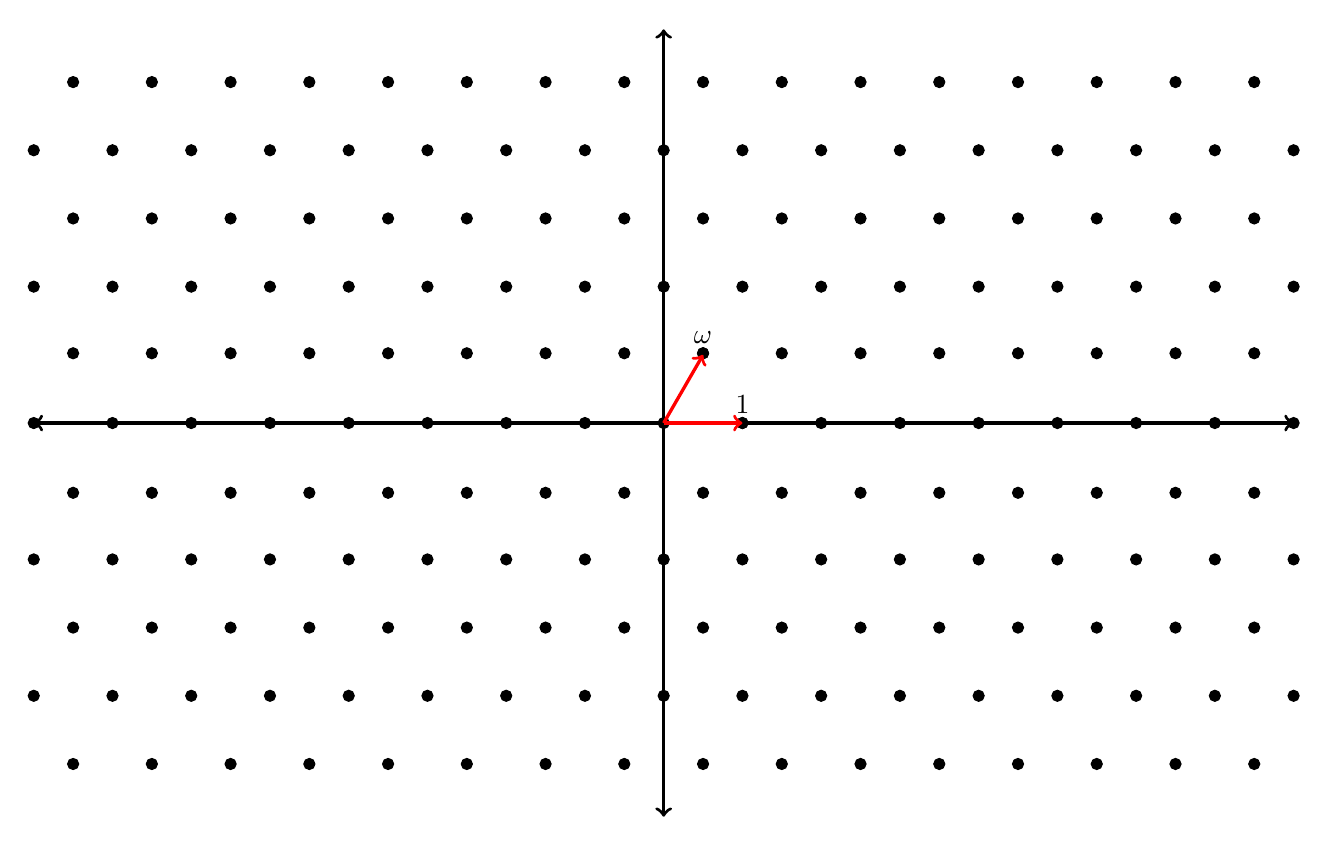
\begin{tikzpicture}
    \draw[black, very thick, <->] (-8,0) -- (8,0);
    \draw[black, very thick, <->] (0,-5) -- (0,5);
    
    \filldraw[black] (1,0) circle (2pt) node[anchor=south] {1};
    \filldraw[black] (.5,.886) circle (2pt) node[anchor=south] {$\omega$};
    
    \filldraw[black] (-8,0) circle (2pt);
    \filldraw[black] (-7,0) circle (2pt);
    \filldraw[black] (-6,0) circle (2pt);
    \filldraw[black] (-5,0) circle (2pt);
    \filldraw[black] (-4,0) circle (2pt);
    \filldraw[black] (-3,0) circle (2pt);
    \filldraw[black] (-2,0) circle (2pt);
    \filldraw[black] (-1,0) circle (2pt);
    \filldraw[black] (0,0) circle (2pt);
    \filldraw[black] (1,0) circle (2pt);
    \filldraw[black] (2,0) circle (2pt);
    \filldraw[black] (3,0) circle (2pt);
    \filldraw[black] (4,0) circle (2pt);
    \filldraw[black] (5,0) circle (2pt);
    \filldraw[black] (6,0) circle (2pt);
    \filldraw[black] (7,0) circle (2pt);
    \filldraw[black] (8,0) circle (2pt);
    
    \filldraw[black] (-7.5,.886) circle (2pt);
    \filldraw[black] (-6.5,.886) circle (2pt);
    \filldraw[black] (-5.5,.886) circle (2pt);
    \filldraw[black] (-4.5,.886) circle (2pt);
    \filldraw[black] (-3.5,.886) circle (2pt);
    \filldraw[black] (-2.5,.886) circle (2pt);
    \filldraw[black] (-1.5,.886) circle (2pt);
    \filldraw[black] (-0.5,.886) circle (2pt);
    \filldraw[black] (0.5,.886) circle (2pt);
    \filldraw[black] (1.5,.886) circle (2pt);
    \filldraw[black] (2.5,.886) circle (2pt);
    \filldraw[black] (3.5,.886) circle (2pt);
    \filldraw[black] (4.5,.886) circle (2pt);
    \filldraw[black] (5.5,.886) circle (2pt);
    \filldraw[black] (6.5,.886) circle (2pt);
    \filldraw[black] (7.5,.886) circle (2pt);
    
    \filldraw[black] (-8,1.732) circle (2pt);
    \filldraw[black] (-7,1.732) circle (2pt);
    \filldraw[black] (-6,1.732) circle (2pt);
    \filldraw[black] (-5,1.732) circle (2pt);
    \filldraw[black] (-4,1.732) circle (2pt);
    \filldraw[black] (-3,1.732) circle (2pt);
    \filldraw[black] (-2,1.732) circle (2pt);
    \filldraw[black] (-1,1.732) circle (2pt);
    \filldraw[black] (0,1.732) circle (2pt);
    \filldraw[black] (1,1.732) circle (2pt);
    \filldraw[black] (2,1.732) circle (2pt);
    \filldraw[black] (3,1.732) circle (2pt);
    \filldraw[black] (4,1.732) circle (2pt);
    \filldraw[black] (5,1.732) circle (2pt);
    \filldraw[black] (6,1.732) circle (2pt);
    \filldraw[black] (7,1.732) circle (2pt);
    \filldraw[black] (8,1.732) circle (2pt);
    
    \filldraw[black] (-7.5,2.598) circle (2pt);
    \filldraw[black] (-6.5,2.598) circle (2pt);
    \filldraw[black] (-5.5,2.598) circle (2pt);
    \filldraw[black] (-4.5,2.598) circle (2pt);
    \filldraw[black] (-3.5,2.598) circle (2pt);
    \filldraw[black] (-2.5,2.598) circle (2pt);
    \filldraw[black] (-1.5,2.598) circle (2pt);
    \filldraw[black] (-0.5,2.598) circle (2pt);
    \filldraw[black] (0.5,2.598) circle (2pt);
    \filldraw[black] (1.5,2.598) circle (2pt);
    \filldraw[black] (2.5,2.598) circle (2pt);
    \filldraw[black] (3.5,2.598) circle (2pt);
    \filldraw[black] (4.5,2.598) circle (2pt);
    \filldraw[black] (5.5,2.598) circle (2pt);
    \filldraw[black] (6.5,2.598) circle (2pt);
    \filldraw[black] (7.5,2.598) circle (2pt);
    
    \filldraw[black] (-8,3.464) circle (2pt);
    \filldraw[black] (-7,3.464) circle (2pt);
    \filldraw[black] (-6,3.464) circle (2pt);
    \filldraw[black] (-5,3.464) circle (2pt);
    \filldraw[black] (-4,3.464) circle (2pt);
    \filldraw[black] (-3,3.464) circle (2pt);
    \filldraw[black] (-2,3.464) circle (2pt);
    \filldraw[black] (-1,3.464) circle (2pt);
    \filldraw[black] (0,3.464) circle (2pt);
    \filldraw[black] (1,3.464) circle (2pt);
    \filldraw[black] (2,3.464) circle (2pt);
    \filldraw[black] (3,3.464) circle (2pt);
    \filldraw[black] (4,3.464) circle (2pt);
    \filldraw[black] (5,3.464) circle (2pt);
    \filldraw[black] (6,3.464) circle (2pt);
    \filldraw[black] (7,3.464) circle (2pt);
    \filldraw[black] (8,3.464) circle (2pt);
    
    \filldraw[black] (-7.5,4.33) circle (2pt);
    \filldraw[black] (-6.5,4.33) circle (2pt);
    \filldraw[black] (-5.5,4.33) circle (2pt);
    \filldraw[black] (-4.5,4.33) circle (2pt);
    \filldraw[black] (-3.5,4.33) circle (2pt);
    \filldraw[black] (-2.5,4.33) circle (2pt);
    \filldraw[black] (-1.5,4.33) circle (2pt);
    \filldraw[black] (-0.5,4.33) circle (2pt);
    \filldraw[black] (0.5,4.33) circle (2pt);
    \filldraw[black] (1.5,4.33) circle (2pt);
    \filldraw[black] (2.5,4.33) circle (2pt);
    \filldraw[black] (3.5,4.33) circle (2pt);
    \filldraw[black] (4.5,4.33) circle (2pt);
    \filldraw[black] (5.5,4.33) circle (2pt);
    \filldraw[black] (6.5,4.33) circle (2pt);
    \filldraw[black] (7.5,4.33) circle (2pt);
%Down
    \filldraw[black] (-7.5,-.886) circle (2pt);
    \filldraw[black] (-6.5,-.886) circle (2pt);
    \filldraw[black] (-5.5,-.886) circle (2pt);
    \filldraw[black] (-4.5,-.886) circle (2pt);
    \filldraw[black] (-3.5,-.886) circle (2pt);
    \filldraw[black] (-2.5,-.886) circle (2pt);
    \filldraw[black] (-1.5,-.886) circle (2pt);
    \filldraw[black] (-0.5,-.886) circle (2pt);
    \filldraw[black] (0.5,-.886) circle (2pt);
    \filldraw[black] (1.5,-.886) circle (2pt);
    \filldraw[black] (2.5,-.886) circle (2pt);
    \filldraw[black] (3.5,-.886) circle (2pt);
    \filldraw[black] (4.5,-.886) circle (2pt);
    \filldraw[black] (5.5,-.886) circle (2pt);
    \filldraw[black] (6.5,-.886) circle (2pt);
    \filldraw[black] (7.5,-.886) circle (2pt);
    
    \filldraw[black] (-8,-1.732) circle (2pt);
    \filldraw[black] (-7,-1.732) circle (2pt);
    \filldraw[black] (-6,-1.732) circle (2pt);
    \filldraw[black] (-5,-1.732) circle (2pt);
    \filldraw[black] (-4,-1.732) circle (2pt);
    \filldraw[black] (-3,-1.732) circle (2pt);
    \filldraw[black] (-2,-1.732) circle (2pt);
    \filldraw[black] (-1,-1.732) circle (2pt);
    \filldraw[black] (0,-1.732) circle (2pt);
    \filldraw[black] (1,-1.732) circle (2pt);
    \filldraw[black] (2,-1.732) circle (2pt);
    \filldraw[black] (3,-1.732) circle (2pt);
    \filldraw[black] (4,-1.732) circle (2pt);
    \filldraw[black] (5,-1.732) circle (2pt);
    \filldraw[black] (6,-1.732) circle (2pt);
    \filldraw[black] (7,-1.732) circle (2pt);
    \filldraw[black] (8,-1.732) circle (2pt);
    
    \filldraw[black] (-7.5,-2.598) circle (2pt);
    \filldraw[black] (-6.5,-2.598) circle (2pt);
    \filldraw[black] (-5.5,-2.598) circle (2pt);
    \filldraw[black] (-4.5,-2.598) circle (2pt);
    \filldraw[black] (-3.5,-2.598) circle (2pt);
    \filldraw[black] (-2.5,-2.598) circle (2pt);
    \filldraw[black] (-1.5,-2.598) circle (2pt);
    \filldraw[black] (-0.5,-2.598) circle (2pt);
    \filldraw[black] (0.5,-2.598) circle (2pt);
    \filldraw[black] (1.5,-2.598) circle (2pt);
    \filldraw[black] (2.5,-2.598) circle (2pt);
    \filldraw[black] (3.5,-2.598) circle (2pt);
    \filldraw[black] (4.5,-2.598) circle (2pt);
    \filldraw[black] (5.5,-2.598) circle (2pt);
    \filldraw[black] (6.5,-2.598) circle (2pt);
    \filldraw[black] (7.5,-2.598) circle (2pt);
    
    \filldraw[black] (-8,-3.464) circle (2pt);
    \filldraw[black] (-7,-3.464) circle (2pt);
    \filldraw[black] (-6,-3.464) circle (2pt);
    \filldraw[black] (-5,-3.464) circle (2pt);
    \filldraw[black] (-4,-3.464) circle (2pt);
    \filldraw[black] (-3,-3.464) circle (2pt);
    \filldraw[black] (-2,-3.464) circle (2pt);
    \filldraw[black] (-1,-3.464) circle (2pt);
    \filldraw[black] (0,-3.464) circle (2pt);
    \filldraw[black] (1,-3.464) circle (2pt);
    \filldraw[black] (2,-3.464) circle (2pt);
    \filldraw[black] (3,-3.464) circle (2pt);
    \filldraw[black] (4,-3.464) circle (2pt);
    \filldraw[black] (5,-3.464) circle (2pt);
    \filldraw[black] (6,-3.464) circle (2pt);
    \filldraw[black] (7,-3.464) circle (2pt);
    \filldraw[black] (8,-3.464) circle (2pt);
    
    \filldraw[black] (-7.5,-4.33) circle (2pt);
    \filldraw[black] (-6.5,-4.33) circle (2pt);
    \filldraw[black] (-5.5,-4.33) circle (2pt);
    \filldraw[black] (-4.5,-4.33) circle (2pt);
    \filldraw[black] (-3.5,-4.33) circle (2pt);
    \filldraw[black] (-2.5,-4.33) circle (2pt);
    \filldraw[black] (-1.5,-4.33) circle (2pt);
    \filldraw[black] (-0.5,-4.33) circle (2pt);
    \filldraw[black] (0.5,-4.33) circle (2pt);
    \filldraw[black] (1.5,-4.33) circle (2pt);
    \filldraw[black] (2.5,-4.33) circle (2pt);
    \filldraw[black] (3.5,-4.33) circle (2pt);
    \filldraw[black] (4.5,-4.33) circle (2pt);
    \filldraw[black] (5.5,-4.33) circle (2pt);
    \filldraw[black] (6.5,-4.33) circle (2pt);
    \filldraw[black] (7.5,-4.33) circle (2pt);

    \draw[red, very thick, ->] (0,0) -- (1,0);
    \draw[red, very thick, ->] (0,0) -- (.5,.866);
\end{tikzpicture}
\caption{We can visualize $\mathbb{Z}[\omega]$ as a lattice in $\mathbb{Q}(\omega)\subseteq\mathbb{C}$ as above.}
\label{fig:Example}
\end{figure}

The horizontal and vertical axis in Figure 1 are the real and imaginary line respectively. Additionally, the lattice is integrally spanned by the basis vectors $1$ and $\omega$ (the red vectors).\\

\begin{definition}\label{def:Norm}
    Let $\alpha$ be an element of $\mathbb{Q}(\omega)$. The norm map $N:\mathbb{Q}(\omega)\to\mathbb{Q}$ defined by $N:\alpha\mapsto\alpha\bar{\alpha}$.
\end{definition}
\begin{theorem}\label{Thm:PosDef}
    For $\alpha,\beta\in\mathbb{Q}(\omega)$, $N(\alpha\beta) = N(\alpha)N(\beta)$ and $N(a-b\omega) = (a-b\omega)(a-b\bar{\omega}) = a^2+ab+b^2$. Additionally, the norm is a positive definite quadratic form on $\mathbb{Q}(\omega)$ taking values in $\mathbb{Z}[\omega]$ when $\alpha\in\mathbb{Z}[\omega]$.
\end{theorem}
\begin{proof}
    Let $\alpha,\beta\in\mathbb{Q}(\omega)$. Then we have 
    \begin{align*}
        N(\alpha\beta) &= (\alpha\beta)\overline{(\alpha\beta)}\\
        &= (\alpha\beta)(\bar{\alpha}\bar{\beta})\\
        &= (\alpha\bar{\alpha})(\beta\bar{\beta})\\
        &= N(\alpha)N(\beta).
    \end{align*}
    Therefore, $N(\alpha\beta)=N(\alpha)N(\beta)$.
    
    For $\alpha = a-b\omega$, $\bar{\alpha} = (a-b\bar{\omega})$.
    Thus,
    \begin{align*}
        N(\alpha) &= (a-b\omega)(a-b\bar{\omega}) \\
        &= a^2 - ab\omega - ab\bar\omega + b^2\omega\bar{\omega}\\
        &= a^2 + b^2(\omega\bar{\omega}) - ab(\omega + \bar{\omega})\\
        &= a^2 + b^2 + ab,
    \end{align*}
    since $\omega\bar{\omega}=1$ and $\omega + \bar{\omega} = -1$. Therefore $N(a-b\omega) = a^2 +ab +b^2$.
    
    Now to prove $a^2 + ab +b^2$ positive definite for $a,b\in\mathbb{Z}$. Without loss of generality we can assume $0\leq|a|\leq|b|$. Therefore $a^2\leq |ab| \leq b^2$. If $ab\geq0$ then $a^2+ab+b^2$ is obviously positive. So we may assume $ab<0$. Assume $|a|=|b|$, then $a^2-ab = 0$, so $a^2-ab+b^2>0$ for $a=b\not=0$. Otherwise, assume $|a|<|b|$ which gives us $a^2-ab+b^2\geq -ab+b^2>0$. Therefore, for $a,b$ not both zero, $a^2-ab+b^2>0$, so the norm is positive definite.
    
    Finally, $N(\alpha)$ is an element of $\mathbb{Z}$ when $\alpha\in\mathbb{Z}[\omega]$ because $a,b\in\mathbb{Z}$ so $a^2+ab+b^2\in\mathbb{Z}$.
\end{proof}
\begin{theorem}\label{Thm:Subfield}
    $\mathbb{Q}(\omega)$ is a subfield of $\mathbb{C}$ and $\mathbb{Z}[\omega]$ a subring of $\mathbb{Q}(\omega)$.
\end{theorem}
\begin{proof}
    To prove $\mathbb{Q}(\omega)$ a subfield of $\mathbb{C}$, $\mathbb{Q}(\omega)$ must satisfy the following:
    \begin{itemize}
        \item[1)] Nonzero and nonempty: Obviously, $0,1\in\mathbb{Q}(\omega)$ by the definition of $\mathbb{Q}(\omega)$.
        \item[2)] Closed under subtraction: Let $\alpha,\beta\in\mathbb{Q}(\omega)$. Then for $\alpha= a + b\omega$ and $\beta= c + d\omega$ ($a,b,c,d\in\mathbb{Q}$), $\alpha-\beta = (a+b\omega)-(c+d\omega) = (a-c) + (b-d)\omega$. Since $a-c,b-d\in\mathbb{Q}$, we have $\alpha-\beta\in\mathbb{Q}(\omega)$.
        \item[3)] Closed under inverse and multiplication: Let $\alpha,\beta\in\mathbb{Q}(\omega)$ and $\alpha,\beta\not=0$. Let $\alpha=a+b\omega$ and $\beta=c+d\omega$ for $a,b,c,d\in\mathbb{Q}$ such that $a,b$ not both zero and $c,d$ not both zero. Then 
        \begin{align*}
            \alpha^{-1} &= \frac{1}{a+b\omega}\\
            &= \frac{1}{a+b\omega}\cdot\frac{a+b\bar{\omega}}{a+b\bar{\omega}}\\
            &= \frac{(a-b)-b\omega}{a^2-ab+b^2}\\
            \tag{2}&= \frac{a-b}{a^2-ab+b^2} - \frac{b}{a^2-ab+b^2}\omega
        \end{align*}
        which is in $\mathbb{Q}(\omega)$ since $a^2-ab+b^2$ positive definite. Next,
        \begin{align*}
            \alpha\beta &= (a+b\omega)(c+d\omega)\\
            &= ac + (ad+bc)\omega + bd\omega^2\\
            &= ac + (ad+bc)\omega + bd(-\omega-1)\\
            \tag{3}&= (ac-bd) + (ad+bc-bd)\omega
        \end{align*}
        which is also in $\mathbb{Q}(\omega)$. 
    \end{itemize}
    Therefore $\mathbb{Q}(\omega)$ is closed under inverses and multiplication so $\mathbb{Q}(\omega)$ is a subfield of $\mathbb{C}$.\\
    
    Using the same equations as above for subtraction and multiplication, we see that $\mathbb{Z}[\omega]$ is also closed under subtraction and multiplication, so $\mathbb{Z}[\omega]$ is a subring of $\mathbb{Q}(\omega)$.
\end{proof}
\begin{theorem}\label{Thm:Units}
    An element $\alpha\in\mathbb{Z}[\omega]$ is a unit if and only if $N(\alpha) = 1$. Additionally the set of units in $\mathbb{Z}[\omega]$ is $\{\pm1,\pm\omega,\pm\bar{\omega}\}$.
\end{theorem}
\begin{proof}
    Assume that $\alpha\in\mathbb{Z}[\omega]$ is a unit. Then there exists a $\beta\in\mathbb{Z}[\omega]$ such that $\alpha\beta=1$. Then we have $1 = N(1) = N(\alpha\beta) = N(\alpha)N(\beta)$. By Theorem 1.2 we have that $N(\alpha),N(\beta)\in\mathbb{Z}$. Therefore $N(\alpha)|1\Rightarrow N(\alpha)=\pm1$.
    
    Next, assume that $N(\alpha)=1$, since $N(\alpha)\geq0$. Then $\alpha = a +b\omega$ implies that $a^2-ab+b^2=1$ and the only integral way for this to equal one is for $(a,b)$ pairs $(\pm1,0),(0,\pm1)$ or $(\pm1,\pm1)$. This is true because $|a|,|b|>1$ implies that $N(\alpha)>1$. And $(a,b)=(1,-1)$ or $(-1,1)$ imply that $N(\alpha)>1$. Plugging each of our $(a,b)$ pairs into equation (2) we find that each of these elements have an inverse in $\mathbb{Z}[\omega]$. Therefore $\alpha$ is a unit.
    
    As explained above, $U= \{\pm1,\pm\omega,\pm(-\omega-1)\}$ is the set of all possible $(a,b)$ pairs such that $a^2-ab+b^2=1$, so $U$ contains all the units of $\mathbb{Z}[\omega]$.
\end{proof}
\begin{theorem}\label{Thm:DivAlg}
    $\mathbb{Z}[\omega]$ has a division algorithm with respect to it's norm map $N$. 
\end{theorem}
\begin{proof}
    Let $\alpha,\beta$ be elements of $\mathbb{Z}[\omega]$. Then to define a division algorithm we show the equation:
    $$\alpha = \delta\beta + \gamma$$
    holds for some $\delta\in\mathbb{Z}[\omega]$ and some $\gamma\in\mathbb{Z}[\omega]$ such that $N(\gamma)<N(\beta)$.
    
    Let $\Delta=\alpha\beta^{-1}=x+y\omega$ be an element of $\mathbb{Q}(\omega)$ and define $\delta := \lfloor x\rceil + \lfloor y\rceil\omega \in \mathbb{Z}[\omega]$. Where $\lfloor \cdot\rceil$ maps rationals to the nearest integer (upwards when equal to $n+1/2$ for some $n\in\mathbb{Z}$). Let $\gamma=\alpha-\delta\beta$. Then we can rewrite $\delta$ as $(x-k) + (y-l)\omega$ for some $-1/2 \leq k,l < 1/2$. Hence,
    \begin{align*}
        \gamma &= \alpha - \delta\beta \in \mathbb{Z}[\omega]\\
        &= \alpha - ((x-k) + (y-l)\omega)\beta\\
        &= \alpha - (\Delta - (k + l\omega))\beta\\
        &= \alpha - \Delta\beta - (k+l\omega)\beta\\
        &= (k+l\omega)\beta 
    \end{align*}
    implies that $N(\gamma) = N(k+l\omega)N(\beta)$. Then, since $|k|,|l|\leq1/2$, $k^2+kl+l^2 \leq 3/4 < 1$. Therefore $N(\gamma) < N(\beta)$ and we have a division algorithm with respect to the norm $N$.
\end{proof}
\begin{definition}\label{Def:Divisibility}
    Let $\alpha,\beta\in\mathbb{Z}[\omega]$. We say $\alpha$ \textit{divides} $\beta$, denoted $\alpha | \beta$, iff there exists a $\delta\in\mathbb{Z}[\omega]$ such that $\alpha\delta=\beta$. (Note: $\delta$ may equal a unit, if so, we call $\alpha$ and $\beta$ \textit{associates}).
\end{definition}

Combining our new definition of divisibility and Theorem 5 gives us 2 very useful corollaries about $\mathbb{Z}[\omega]$.

\begin{corollary}\label{Cor:UFD}
    $\mathbb{Z}[\omega]$ is a unique factorization domain.
\end{corollary}
\begin{proof}
    Theorem 5 shows that $\mathbb{Z}[\omega]$ is a euclidean domain because $N(\alpha)\leq N(\alpha\beta)=N(\alpha)N(\beta)$ for nonzero $\alpha,\beta\in\mathbb{Z}[\omega]$. And we know that every principal ideal domain is a unique factorization domain, so we just need to prove that all euclidean domains are principal ideal domains. 
    
    Let $I$ be an ideal of a euclidean domain $D$ with norm $d$. Then, assume that $I\not=\langle 0 \rangle =\{0\}$. Assume that $a$ is a nonzero element in $I$ such that $d(a)$ is minimal. Then assume that $b\in I$ as well. We can then write $b = na+r$ for $d(r)<d(a)$ by the division algorithm defined on $D$. If $r\not=0$, then $r$ a nonzero element of $I$ such that $d(r)<d(a)$ which is a contradiction, so $r=0$. Therefore $a | b$ and $b\in\langle a\rangle$. Therefore every ideal in $D$ is principal. It then follows that $D$ is also a unique factorization domain.
\end{proof}
\begin{corollary}\label{Cor:PrimeIrred}
    Let $\alpha$ be an element of $\mathbb{Z}[\omega]$. Then, $\alpha$ is prime if and only if $\alpha$ is irreducible.
\end{corollary}
\begin{proof}
    Remember that $\mathbb{Z}[\omega]$ is a UFD by Corollary 5.1. Assume that $\alpha$ is irreducible, then $\alpha=p_1\dots,p_n$ is a unique prime factorization of $\alpha$, however, since $\alpha$ is irreducible, $n>1$ gives a contradiction. Therefore $\alpha = p_1$ so $\alpha$ is prime. Assume that $\alpha$ is prime and $\alpha = \beta\gamma$. Then, without loss of generality, we may assume $\beta=\alpha\delta$ for some $\delta\in\mathbb{Z}[\omega]$. So $\alpha = \alpha\delta\gamma$, which implies that $\delta^{-1}=\gamma$ so $\delta$ and $\gamma$ are both units in $\mathbb{Z}[\omega]$, so $\alpha$ is irreducible.
\end{proof}
\begin{definition}\label{Def:GCD}
    The \textit{greatest common divisor} of two elements $\alpha,\beta\in\mathbb{Z}[\omega]]$ is the element $\delta$ such that $\delta | \alpha$ and $\delta | \beta$, and $\gamma|\alpha$ and $\gamma|\beta$ imply that $\gamma|\delta.$ The greatest common divisor of $\alpha$ and $\beta$ is denoted $\gcd(\alpha,\beta)$.
\end{definition}
\begin{corollary}\label{Cor:GcdExist}
    Every pair $\alpha,\beta$ have a greatest common denominator. However, this gcd is not unique, and may differ by units of $\mathbb{Z}[\omega]$.
\end{corollary}
\begin{proof}
    
\end{proof}
\begin{theorem}\label{Thm:Bezout}
    Let $\alpha,\beta\in\mathbb{Z}[\omega]$. Then, there exists $\delta,\gamma\in\mathbb{Z}[\omega]$ such that
    $$\delta\alpha + \gamma\beta = \gcd(\alpha,\beta).$$
\end{theorem}
\begin{proof}
    Assume that $\beta$ does not divide $\alpha$. We may proceed iteratively with the division algorithm above to get the following:
    \begin{align*}
        \alpha &= \beta \delta_1 + \gamma_1  &&0<N(\gamma_1)<N(\beta)\\
        \beta &= \gamma_1\delta_2 + \gamma_2  &&0<N(\gamma_2)<N(\gamma_1)\\
        \vdots\\
        \gamma_{n-2} &= \gamma_{n-1}\delta_{n} + \gamma_{n}  &&0<N(\gamma_{n})<N(\gamma_{n-1})\\
        \gamma_{n-1} &= \gamma_{n}\delta_{n+1}.
    \end{align*}
    We know that the algorithm terminates because the norm is finite and strictly decreasing on the integers. Fix $n$ as the minimum required $\gamma_i$ as seen above until termination. Since $\Delta=\gcd(\alpha,\beta) | \alpha$ and $\Delta|\beta$, we know that $\Delta$ must divide $\gamma_1$ and similar reasoning for $\Delta | \gamma_2$. Then, assume $\Delta | \gamma_{i-2}$ and $\Delta | \gamma_{i-1}$, then $\Delta$ must divide $\gamma_i$ by the above list of equations. Therefore, $\Delta$ divides $\gamma_i$ for $i=1,2,\dots,n$.
    
    Since $\gamma_n | \gamma_{n-1}$, we have $\gamma_n | \gamma_{n-2}$. Next, assume $\gamma_n | \gamma_{i+2}$ and $\gamma_n | \gamma_{i+1}$. Then, $\gamma_n | \gamma_i$ for all $\gamma_i$ for $i=1,2,\dots,n$. We can then further this to say $\gamma_n | \beta$ and $\gamma_n | \alpha$. By the definition of $\gcd(\alpha,\beta),$ $\gamma_n | \Delta$.
    
    Thus, by both of these inductive arguments, $\gamma_n = \Delta = \gcd(\alpha,\beta)$.
    
    Assume that $\Delta$ can be written as a linear combination of $\gamma_n$ and $\gamma_{n-1}$, then $\Delta$ can also be written as a linear combination of $\gamma_{n-1}$ and $\gamma_{n-2}$ as follows:
    \begin{align*}
        \Delta = \gamma_{n+1} &= \gamma_{n-1}-\gamma_n\delta_{n+1}\\
        &= \gamma_{n-1}-(\gamma_{n-2}-\gamma_{n-1}\delta_n)\delta_{n+1}
    \end{align*}
    Then, $\Delta$ can be written as a linear combination of $\gamma_1$ and $\gamma_2$. Therefore, since we can write $\gamma_1=\alpha-\beta\delta_1$ and $\gamma_2 = \beta - (\alpha-\beta\delta_1)\delta_2 = (1+\delta_1\delta_2)\beta - \alpha\delta_2$, $\Delta=\gcd(\alpha,\beta)$ may be written as a linear combination of $\alpha$ and $\beta$.
\end{proof}




\begin{theorem}
    A rational prime $p$ can be written $p=m^2+mn+n^2$ for some $m,n\in\mathbb{Z}$ if and only if $p\equiv -1 \mod{3}$.
\end{theorem}
\begin{proof}
    Let $p$ be a rational prime. For $p$ to be a $\omega$-prime, there must be no $\alpha\in\mathbb{Z}[\omega]$ such that $N(\alpha)|p$ where $1<N(\alpha)$. Therefore, $p$ is $\omega-$prime if and only if $p\not=m^2+mn+n^2$ for any $m,n\in\mathbb{Z}$. Additionally, a $\omega$-prime, $\pi$ has norm $p$ if and only if $p$ is not $\omega-$prime. So $\pi$, where $N(\pi)=p$, is prime if and only if $p=m^2+mn+n^2$ for some $m,n\mathbb{Z}$. 
    
    Assume $p\equiv 0\mod{3}$, then $p$ must be equal to 3. However, $3=1^2 + 1(-2) + (-2)^2 = (1-2\omega)(1-2\bar{\omega})$ so 3 is not prime in $\mathbb{Z}[\omega]$. So $p$ must be congruent to $-1$ or $1$ modulo $3$.
    
    Assume $p=m^2+mn+n^2$ and $p\not=3$. Then we have $p=(m-n\omega)(m-n\bar{\omega})\Rightarrow p/n^2 = (m/n)^2 + (m/n) + 1$. (This is because $n\not=0$ due to $p$ being prime). Therefore, since $n,p$ coprime, $n\in U_p$. so there exists some $x>1\in\mathbb{N}$ such that $n^{x}\equiv 1 \mod{p}$ (choose $x$ such that $n^{x-1}=n^{-1}$ which exists by coprime. Multiply the entire equation by $n^{2x}$ to get 
    \begin{align*}
        pn^{2x-2} &= m^2n^{2x-2} + mn^{2x-1} + n^{2x}\\
        &= m^2n^{2x-2} + mn^{2x-1} + (n^{2x} - 1) + 1
    \end{align*}
    Which we can subtract $n^{2x}-1$ from both sides to get
    \begin{align*}
        pn^{2x-2} - (n^{2x}-1) &= m^2n^{2x-2} + mn^{2x-1} + 1\\
        &= (mn^{x-1})^2 + mn^{2x-1} + 1\\
        &= (mn^{x-1})^2 + mn^xn^{x-1} + 1.
    \end{align*}
    Then, since $n^x\equiv 1 \mod{p}$ and $n^{2x}-1\equiv 0 \mod{p}$, $$pn^{2x-2} - (n^{2x}-1) \equiv 0 \equiv (mn^{x-1})^2 + mn^{x-1} + 1 \mod{p}$$
    So we have $p | a^2 + a + 1$ for $a=mn^{x-1}\in\mathbb{Z}$. This implies that $p|(a+\frac{1}{2})^2+\frac{3}{4}$ which implies $p|4\cdot\left[(a+\frac{1}{2})^2+\frac{3}{4}\right] = (2a+1)^2 + 3$ or $(2a+1)^2\equiv -3\mod{p}$. Then we have $(-3\mid p)=1$ for $p$ and 3 coprime. Because we assumed $p\not=3$, by quadratic reciprocity we have 
    \begin{align*}
        \left(\frac{p}{-3}\right)\left(\frac{-3}{p}\right) = (-1)^{\frac{p-1}{2}\frac{-3-1}{2}}&=1,\\
    \end{align*}
    which gives us
    \begin{align*}
        \tag{4}\left(\frac{-3}{p}\right) = \left(\frac{p}{-3}\right) = 1.
    \end{align*}
    Therefore, $p=m^2+mn+n^2$ for some $m,n\in\mathbb{Z}$ implies that -3 is a quadratic residue modulo $p$. So $(p\mid -3)=-1$ implies that $p$ is prime in $\mathbb{Z}[\omega]$ because $p$ doesn't equal $m^2+mn+n^2$ for any $m,n\in\mathbb{Z}$. Assume $p\equiv -1 \mod{3}$, then it is fairly easy to check that $p$ has no quadratic residues mod 3: $$0^2\equiv0,\, 1^2\equiv1,\,2^2\equiv1 \Mod 3.$$ None of which are congruent to $-1$. Therefore $(p\mid -3)=-1$ and $p$ is prime in $\mathbb{Z}[\omega]$.
    
    Assume $p\equiv 1 \mod{3}$. Then $(-3\mid p) = 1$ because $p\equiv 1 \Mod3$ has quadratic residue 1 and because of equation (4). Let $b\in\mathbb{Z}$ such that $b^2\equiv -3 \Mod p$. Then, since $2$ coprime to $p$, let $a \equiv 2^{-1}(b-1)\Mod p$. Then $b \equiv 2a+1$ and 
    \begin{align*}
        0 &\equiv b^2+3\\
        &\equiv (2a+1)^2+3\\
        &\equiv 4(a^2+a+1).
    \end{align*}
    $p$ is prime, so $p$ does not divide 4. Therefore, $p\mid a^2+a+1 = (a-\omega)(a-\bar{\omega}).$ Since $p$ obviously doesn't divide $a-\omega$ or $a-\bar{\omega}$ due to $p \nmid a$ (since $p\mid a^2+a+1$) and $p\nmid 1$ (since $p$ is prime). We then have that $p$ is composite in $\mathbb{Z}[\omega]$.
    
    All cases of $p\equiv 0,1,-1 \Mod p$ have been covered, and $p$ is prime if $p\equiv -1\Mod 3$ and composite otherwise. Therefore, $p$ is $\omega$-prime if and only if $p\equiv -1 \mod{3}$.
\end{proof}

\begin{theorem}
    Let $k$ be a rational integer such that $k=m^2+mn+n^2$ for some $mn,\in\mathbb{Z}$. Then $k$ is of the form $$k = 3^cp_1^{a_1}p_2^{a_2}\dots p_k^{a_k}q_1^{2b_1}q_2^{2b_2}\dots q_l^{2b_l}$$ for $p_i\equiv 1\Mod3$ prime, $q_i\equiv -1 \Mod3$ prime, and $a_i,b_i,c\in\mathbb{Z}$.
\end{theorem}
\begin{proof}
    Let $k$ be a rational integer and assume $k=m^2+mn+n^2$ for some integers $m,n$. By this assumption, there exists a $\pi\in\mathbb{Z}[\omega]$ such that $N(\pi)=k$. Since $\mathbb{Z}[\omega]$ is a UFD, let $\pi = (1-2\omega)^c\alpha_1^{a_1}\alpha_2^{a_2}\dots\alpha_k^{a_k}q_1^{b_1}q_2^{b_2}\dots q_l^{b_l}$ be the prime factorization of $\pi$ in $\mathbb{Z}[\omega]$ where $N(\alpha_i)=p_i\equiv 1 \Mod3$ and $q_i\equiv -1 \Mod 3$ for $a_i,b_i\in\mathbb{Z}$ (by Theorem 7). Then, $k=N(\pi)=N((1-2\omega)^c)N(\alpha_1^{a_1})N(\alpha_2^{a_2})\dots N(\alpha_k^{a_k})N(q_1^{b_1})N(q_2^{b_2})\dots N(q_l^{b_l})$. Then, $k=3^cp_1^{a_1}p_2^{a_2}\dots p_k^{a_k}q_1^{2b_1}q_2^{2b_2}\dots q_l^{2b_l}$ for $p_i\equiv 1\Mod 3$ and $q_i\equiv -1\Mod3$. Then, to show that $k$ cannot be divided by some $q_*\equiv -1 \Mod3$ and not $q_*^2$ assume that $p_*$ divides $k$. Then, since $p_*$ is prime,$p_*$ divides one of $3,N(\alpha_i),$ or $N(q_i)$ as defined above. However, $p_*$ cannot divide $3$ nor $N(\alpha_i)$ for any $\alpha_i$ because $N(\alpha_i)\equiv 1 \Mod3$ and prime. Therefore, $p_*$ must divide $N(q_{i_0})$ for some $i_0$. But, since $N(q_{i_0})$ is a square, $p_*|N(q_{i_0})$ implies that $p_*^2|N(q_{i_0})$. Therefore, every integer $k$ that can be written $k=m^2+mn+n^2$ is of the form
    $$k = 3^cp_1^{a_1}p_2^{a_2}\dots p_k^{a_k}q_1^{2b_1}q_2^{2b_2}\dots q_l^{2b_l}$$
    for $p_i\equiv 1\Mod3$ prime, $q_i\equiv -1 \Mod3$ prime, and $a_i,b_i,c\in\mathbb{Z}$.
\end{proof}

\section*{Computation Notes}
I created a python(sage) program to test my conjecture in Theorem 7. To do this, I created an ordered list of every single prime $p$ that could be written $p=m^2+mn+n^2$ for some $-1000\leq m,n\leq 1000$. I then created an ordered list of every single prime congruent to $1$ mod 3. After this I tested to see how many indices these two lists agreed without disagreeing once (other than 3 in the first list) and it came that they agree for the first 39351 terms. This is equivalent to saying that the first 39351 primes congruent to 1 mod 3 can be written as the sum $m^2+mn+n^2$ for some integers $m,n$ in the range $[-1000,1000]$.
\end{document}